\documentclass[12pt]{article}
\usepackage{preamble}

\pagestyle{fancy}
\fancyhead[LO,LE]{Физические основы компьютерных \\ и сетевых технологий}
\fancyhead[RO,RE]{Лекции Зинчика А. А.}

\fancyfoot[L]{\scriptsize исходники найдутся тут: \\ \url{https://github.com/pelmesh619/itmo_conspects} \Cat}

\renewcommand{\thesection}{}

\begin{document}

    \tableofcontents
    \clearpage

    % begin physics3_2025_09_01.tex





\section{Поляризация}

В прошлом семестре мы говорили о плоских бесконечных волнах. В реальности волны не бесконечные -- о них говорят, как о импульсе, одиночном, кратковременном возмущении

Свет излучается атомами за конечное время, порядка наносекунд. Получаем конечный световой импульс, длину распространения которого можно посчитать -- $l = c \cdot t$, а значит мы можем говорить о световом импульсе, который локализован, как о частице. Здесь появляется понятие кванта: атом не может излучить меньше одного фотона, поэтому фотон -- это квант, неделимая часть

Из прошлого семестра мы знаем, что электрон может преодолеть потенциальный барьер, действуя как волна, из-за своего размера. Следствием этого является ограничением на размер транзистора

Такой эффект не сходится с представлениями классической физики. В классической физике (в том числе в механике Ньютона) рассматриваются более высокие порядки размеров и на более низких скоростях, чем скорость света.
В механике Гамильтона, основывающейся на концепции гамильтониана (оператора полной энергии) отпадает понятие траектории

\mediumvspace

Будем говорить, что волна представляет $E(z, t) = \RE(E_0 e^{i(\omega t - kz)})$

Если волна не лежит в системе координат, то добавляют матрицу поворота: $E(z, t) = \RE\left(E_0 \begin{pmatrix}\cos \theta \\ \sin \theta \end{pmatrix} e^{i(\omega t - kz)}\right)$

\smallvspace

Свет считается \textbf{поляризованным}, если направления колебания светового вектора $\vec E$ упорядочены каким-либо образом

% TODO картинка

В простом случае поляризация бывает линейной (или плоской) -- в этом случае вектор напряженности движется в одной плоскости

Большинство бытовых источников света излучают неполяризованные волны -- в них колебания разных направлений быстро и беспорядочно сменяют друг друга. С помощью устройства с названием \textbf{поляризатор} можно получить поляризованный свет, поглощая другие. Поляризатор лишь частично задерживающий колебания, перпендикулярные к его плоскости, называется несовершенным. Качество поляризатора зависит от толщины и материала

С помощью другого прибора -- монохроматора -- можно получить монохроматическую волну. Так как свет с разной длиной волны имеет разные коэффициенты преломления, то монохроматор способен пропускать свет с нужной длиной волны

Если свет поляризован плохо, то его называют \textbf{частично поляризованным}

% TODO картинка

Если пропустить частично поляризованный свет через поляризатор, прибора вокруг направления луча интенсивность прошедшего света будет изменяться от $I_\min$ до $I_\max$. Причем, так как поляризатор симметричен, то угол между $I_\min$ и $I_\max$ равен $\frac{\pi}{2}$

Степенью поляризации $P = \frac{I_{\max} - I_\min}{I_{\max} + I_\min}$ можно выразить, насколько сильно поляризован свет 

\mediumvspace

Однако, так как поляризатор не пропускает лучи в неправильном направлении, то интенсивность света уменьшиться. \textbf{Закон Малюса} гласит, что доля интенсивность выходящего света от интенсивность входящего равна $\cos^2 \varphi$, где $\varphi$ -- угол между плоскостью поляризатора и плоскостью колебания $\vec E$

\[I = I_0 \cos^2 \varphi\]

Если пропустить естественный свет через поляризатор, то интенсивность выходящего света равна $I = \frac{1}{2} I_0$. Это объясняется тем, что в естественном свете волны направлены во все стороны равновероятно, а среднее значение $\cos^2 \varphi$ равна $\frac{1}{2}$

\mediumvspace

Существует круговая (или эллиптическая) поляризация, когда вектор $\vec E$ вращается в плоскости, перпендикулярной направлению распространения волны


% end physics3_2025_09_01.tex

% begin physics3_2025_09_08.tex





Всего существуют 3 способа поляризации:

\begin{enumerate}
    \item Поглощение (или дихроизм): свет проходит через вещество с длинными нитевидными молекулами. Проходя вдоль молекулы, свет свободно проходит, а поперек молекул свет не проходит

    Большинство таких линейных поляризаторов (или так называемых поляроидов) состоят из полимерной пленки или частиц кристаллов турмалина или герапатита в нитроцеллюлозной пленке

    \item Преломление: в призме Николя используется двойное лучепреломления света. В ней используется анизотропный кристалл исландского шпата, в котором

    \begin{itemize}
        \item лучи, поляризованные горизонтально, имеют показатель преломления $n_o = 1.66$ -- их называют обыкновенными
        \item лучи, поляризованные вертикально, имеют показатель преломления $n_o = 1.51$ -- их называют необыкновенными
    \end{itemize}

    Призма Николя представляет собой две одинаковые треугольные в сечении призмы. Обыкновенный луч испытывает полное внутреннее отражение от склеивающего слоя с $n = 1.55$ и поглощается, а необыкновенный свободно проходит через него и вторую призму, так как показатели преломления приблизительно равны

    % TODO картинка

    \item Отражение: Столетов предложил сделать поляризатор из стекла. При определенном угле падения $\alpha = \arctg n$ (известном как угол Брюстера) отраженный свет получается поляризованным. Для стекла этот угол равен примерно $59^{\circ}$, однако отраженный свет получается с интенсивностью 4\% от интенсивности входящего света.

    Столетов предложил использовать несколько стеклянных пластин, чтобы увеличить интенсивность -- данное устройство, состоящее из стопки стекла, получило название стопа Столетова

    Угол Брюстера применяется в изготовлении лазеров для получения поляризованных волн 

    % TODO картинка
\end{enumerate}

\section{Дисперсия света}

Дисперсией света называется зависимость показателя преломления от частоты волны света

Данных эффект был обнаружен Исааком Ньютоном при разложении света в спектр. Тогда Ньютон обнаружил, что для разных частот света (а следовательно для разных волн) показатель преломления разный, поэтому в стекле лучи разных частот двигаются с разной скоростью, на выходе призмы получается радужный спектр 

Благодаря дисперсии существует радуга: лучи Солнца, проходя под определенным углом (42 градуса над горизонтом) через капельки воды в воздухе, раскладываются в спектр и попадают на сетчатку глаза

\begin{wrapfigure}{R}{0pt}
    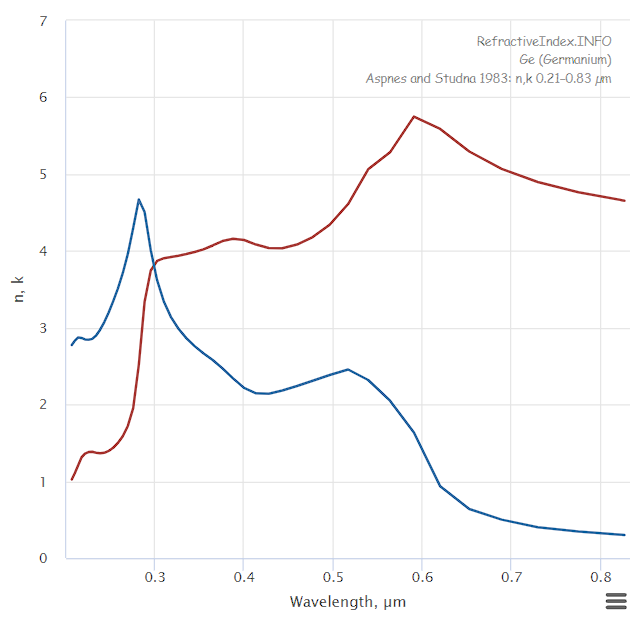
\includegraphics[width=6cm]{physics3/images/physics3_germanium_refractive_index}
\end{wrapfigure}

На сайте \url{https://refractiveindex.info} можно узнать показатель преломления. Например, металл германий, использующийся в тепловизорах, имеет показатель преломления 3.5-4 в инфракрасном спектре волн, что улучшает разрешение тепловизора при ограниченном объёме устройства

Подобные призмы используются в спектрометрах - приборах, позволяющих разложить свет в спектр и узнать, какие длины волн пресутсвуют в спектре

Разные газы в газоразрядной лампе излучают свет разного цвета (то есть спектр из разных длин волн). Поэтому с помощью спектрометра можно обнаружить, из чего состоит источник света (например, Солнца): зная спектр горения водорода и гелия, можно предположить концентрацию горящего вещества на поверхности Солнца

Более продвинутый прибор -- масс-спектрометр -- используется для изучения состава вещества: вещество нагревают, излученный свет попадает на масс-спектрометр, который определяет интенсивность для разных волн света

% NO ANTI-MASS SPECTROMETER? 😿 
% @@@%%%%%%%%%%%%%%@%@@@@@@@@%%%%%%%%%#%##%%@@@@%%%%%%@@@@@@@%#***#####%%%@@%@@@@@@@@@@@@@%%@@@@@@%@@@
% %%%%%@%%%%%%%%%%%%%%@%@%@@@@%%%%%#%####%@@@@@@@@%%@%@@@@@@@@@@@@%%%%%%%%@@@@@@@@@@@@%%%@@@@%@@@@@@%%
% @%%%%%@%@@%%%%%%%%%%%%%@@@@@%@%%%%%%%##%@%@@@@@@%%@@@@@@@@@@@@@@@%%%%%%%@@@@@@@@@%%%@@@%%%%@@@%@@%@%
% @%%%%%%%%%%%@@%%%%%%%%%%%%%%@%@@%%%%%%@%@%%@@@@%#%@@@@@@@@@@@@@@%###%%@@@@@@@%%%%@@%%%%@@@@@%%%@@%%@
% %%%%%%@@%@%%%%%%%@@%%%%%%%%%%%%@@@@%%%@%@%@@@@@%%%@@@@@@@@@@@@@@@@@@@@%%%%%%%%@%@%@@@@@%%%%@%@%@%%%%
% %%%%%%%@@%%%%%%%%%%%%%@%%%%%%%%%%%%%%@%@@@@@@@@%%%@@@@@@@@@@@@@@@@@@%%%@%@%@@%%@@@%%@%%%%@@%%%%@%%%%
% %%%%%%%%%%@%@%%%%%%%%%%%%%@%%%%%%%%%%@%@%@@@@@@%%%@@@@@@@@@@@@@@@@@@@%%%%%@%@@%%%@%@@%%%%%%%%%%%%%%%
% %@%%%%%%%%%%%%%%%%%%%%%%%%%%%%%@%%%%%@@%@@@@@@@%%%@@@@@@@@@@@@@@@@@@@@@@%%%%@%%%%@%%%%%%%%%%%%%%%@@@
% %%%%%%%%@@@@%%%%%%%%%%%%%%%%%%%%%%%%%@%@%@@@@@@%#%@@@@@@@@@@@@@@@@@@%%@%%%%%%%%%%%%%%%%%%%%%%%@%%%%%
% %%%%%%%%%%%%%%%@@@%%%%%%%%%%%%%%%%%%%@@%@@@@@@@%%%@@@@@@@@@@@@@@@@@@%%%%%%%%%%%%%%%%@@@%%%%%%%%%%%%%
% %%%%%%%%%%%%%%%%%%%%%%%%%%%%%%%%%%%%%@%@%@@@@@@%%%@@@@@@@@@@@@@@@@@@%%%%%%%%%%@@@%%%%%%%%%%%%%%%%%%%
% %%%%%%%%%%%%%%%%%%%%%%%%%%%%%%%%%%%%%@%@%%%%@@@%%%@@@@%%%%%%%%%@@@@%%%@%%@%%%%%%%%%%%%%%%%%%%%%%%%%%
% %%%%%%%%%%%%%%%%%%%%%%%%%%%%%%%%%%%%%@%%%%%%%@@@%#%%@%%%%%%%%%@@@@@%%%%%%%%%%%%%%%%%%%%%%%%%%%%%%%%%
% %%%%%%%%%%%%%%%%%%%%%#%%%%%%%%%%%%%%%%%@%%%%%%%@@%%%%%#####%%@@@%%%%%%%%%%%%%%%%%%%%%%%%%%%%%%%%%%%%
% @@@@%%%%%%%%##%%%%%%%%%%%%%%%%%%%%%%%%%%%%%%%%%%@%%%@%####%@@@%%%%%%%%%%%%%%%%%%%%%%%%%%%%%%%%%%%%%%
% %%%%%%%%%%%%%%%%%%%%%%%%%%%%%%%%%%%%%%%%%%%%%%%%%%#*####%@@%%%%%%%%%%%%%%%%%%%%%##%%%%%%%%%%%%%%%%%%
% %%%%%%%%%%%%%%#####%#*#####%%%%%%%%%%%%%%**#%%%%%%%@@%%%%%####*##%###%%%%%%%%##########%%###%%#%%%%%
% ###%%%%%%%%%#########**#%####%%%%%%%%%#%%***%%%%%%%%%%%@%%####**###*#%#%%%%%%###*######%%###%##%%%%%
% ####%%%%%%%%#########*#*########%%%######===******#%%%*#***##*+*###*#%####%#####*######%%###%#######
% #####%%%%##################%%#####%%#####**+**##%%*==#%%%###***#######%%%%#%%%######################
% #%%%#%%%%####*#%%%##*####*#%%#*##%%%%#*##%%#=*#%%%%=-%%%#*++*%%%######%%%%#%%#*#**#%%#*#*##**#%%%###
% ##%%####%######%%%##***####%%####%%%#######*=*#%%%#=-#%%#***##%#######%%%%#%%%#%%%%%###%####*#%%%###
% #*#%%######%%##%%%##**################*#####*+*####-=*%%%**#%%%#######%%%##%####**#%%%%%%#%%#%%%%%%#
% #%%%%###%%#%%%%#####*****##***#*######***##%#*+*#%*==##%%**###%%%######%#######***#######****#%%####
% ##%%%#######%%######**##**##%%#**##%#**%#*****++*#*==#****+*####%%#*##%%%%%###******##******######%%
% #%%%%####%######*#####*****###***#*#***##*****=*##*==#+***++***#%##**####*#%#****###*#*****######%##
% #############%%%%%%#*******************##***##*#%#+:=*****++**#*%#****###**##*****#%##****#*****####
% #######%##**########********#*+++***************%%*::=*****#######**++++**###******#*******#%%#*####
% #*##%%##*#****####********+++******************+=**:-++***%%%%%%%*****#%%**++***************#%%####*
% #*##%#****#*##**###**+++****%%%***#%%##***++*##+=*=.-=-:-=+++**++**#%%%##%##**+==+**********#####*##
% #*######%###*##**++*****#%%%%%%#%#%####%%%*++*#*=++::=+*#*+*+++==#*#########%##*+=====********###***
% ****#**#*#*#++*******%%%#%%#**#*+#%%+++******#%##==:-:=#@*#@%*+****+#**#***###*#%#**++===+*##%#*##*#
% ***#*#%%@@%@%%%%%#********++++===*%%*===*****%%@%*=:+**#%%%*+==*#%#%#%%%%%%%%%#%%%%%*#***+++++*##***
% ****#%@%%%%%%%%%*+*#******++===++*%%%****##****%%*+:=%*#%***+*#%*#%%%%%%%%%%%%%#%######%%##****++***
% ***%@%%%%%%%%%%*=+#%%%%#***#*+++++%@%%%##%%%%%%@@@#:+****##%%%%***%%%%%*#******%%########%#%%#*****+
% ##%%%%%%%%%%#%*=+*#%%#*******++++*#@@@@%%%%%%%%@@@%*###**#%%%%%@*#%##*+*****====+++***********######
% %@%%%%%%%%%%%*=+*#%%**************#%%%%%%%%%%%%%%%%@%##**#%%%%%@@%%**++++***=====+++*************#*#
% %%%%%%%%%%%%*=+**%#***********+==**%%%%%%%##%@%%%%%%%%#%#%%%%%##%%#****+*+=+==+*%*###**************#
% %%%%%%%%%%%+=+*#%%*****++*******+**##*##*#%%%%%%%%%@@%%@%%%%%%#*=---=*##*+:===+*#*****%#%#%%%@%*****
% %%%%%%%#%%*=++*#%#*********************+++*##*=*####**%@%%%@@%******+==--=*%===#%##*#*%#%%####%%#***
% %%%%%%#%%*=++*#%#**********+*++++++++++++**#+-=*##**##%@@@@@%#*++++***++**+====*#####%%%#%%%%%%%%#**
% %%%%%%%%+=++*#%%***********+++++++++++*****=-=******##%%@@@%%%#*****#***+**+===*#%*#**#%#%%%%%%%%%#*
% %%%%#%%+=++*##%%*******+=====+++++++++**#*=-=*#**+++*##%%%%%%#******+++****+====+**%#%%%@%%#%%%%@%%#
% %%%@%%*=++**#%%%****++===========++=+*##*--=+***++++*##*##%%%******++++++**#*+====+++*%#%%%%%%%%#%%@


Дисперсия возникает как следствие уравнение Максвелла. Допустим для слабопроводящей среды $\sigma, \varepsilon, \mu = \const$ ($\sigma = \frac{1}{\rho}$ -- удельная проводимость в сименсах)

По закону индукции Фарадея $\vec\nabla \times \vec E = -\mu\mu_0 \frac{\partial \vec H}{\partial t}$

$\nabla \times (\nabla \times \vec E) = -\mu\mu_0 \frac{\partial}{\partial t} (\nabla \times \vec H)$

$\nabla \times (\nabla \times \vec E) = \nabla (\nabla \vec E)$

$\nabla^2 \times \vec E = -\mu\mu_0 \frac{\partial}{\partial t} (\nabla \times \vec H)$

По теореме о циркуляции магнитного поля $\nabla \times \vec H = \sigma \vec E + \varepsilon \varepsilon_0 \frac{\partial \vec E}{\partial t}$

Получаем $\frac{\partial^2 \vec E}{\partial t^2} + \frac{\sigma}{\varepsilon \varepsilon_0} \frac{\partial \vec E}{\partial t} = v^2 \Delta \vec E$ -- волновое уравнение, где $v^2 = \frac{1}{\varepsilon \varepsilon_0 \mu \mu_0}$

Из этого волнового уравнения для волны, направленной в сторону оси $Ox$, получаем $\frac{\partial^2 E_y}{\partial t^2} = v^2 \Delta E_y - \frac{\sigma}{\varepsilon \varepsilon_0} \frac{\partial E_y}{\partial t}$

Решение его является функция $E_y = E_0 e^{i (\omega t - k x)}$, то есть $\omega^2 = v^2 k^2 - \frac{i \omega \sigma}{\varepsilon \varepsilon_0}$, где $k = \frac{2\pi}{\lambda}$ -- волновое число

Уравнение 

\[k^2 = \frac{\omega}{v^2} - \frac{i \omega \sigma}{\varepsilon \varepsilon_0 v^2}\]

называют дисперсионным (то есть зависимость $k(\omega)$). Из него $k = \pm \frac{\omega}{v} \sqrt{1 - \frac{i \sigma}{\varepsilon \varepsilon_0 \omega}}$

Для $\frac{\omega}{\varepsilon\varepsilon_0 \omega} \ll 1$ можем аппроксимировать корень, получаем $k \approx \frac{\omega}{v} \left(1 - i \frac{\sigma}{2\varepsilon\varepsilon_0 \omega}\right) = k^\prime - i k^{\prime\prime}$

В ходе вычисления получаем комплексное $k$: вещественная часть волнового числа $k^\prime$ определяет длину волны, мнимая часть $k^{\prime\prime} = $ показывается коэффициент затухания волн, то есть поглощение, получаем $E_y = E_0 e^{i (\omega t - k^{\prime} x) - k^{\prime\prime} x}$

Зависимость фазовой скорость волны (то скорость волны с одной длиной) от частоты в среде $v_\text{фаз}(\omega) = \frac{\omega}{k^{\prime}(\omega)}$ называют дисперсией (также обозначают $v_{\text{фаз}} = v$)

Для световых волн дисперсия -- $n(\omega) = \frac{c}{v_{\text{фаз}}(\omega)}$ или $n(\lambda_0) = \frac{c}{v_{\text{фаз}}(\lambda_0)}$

Если $\sigma = 0$, то $v_{\text{фаз}} = \frac{1}{\sqrt{\varepsilon \varepsilon_0 \mu \mu_0}}$

Получаем дисперсию световых волн: $n(\omega) = \frac{c}{v_{фаз}(\omega)}$ или $n(\lambda_0) = \frac{c}{v_{фаз}(\lambda_0)}$

Из этого выходит закон Бугера: пусть свет интенсивности $I_0$ падает на вещество толщины $L$, тогда интенсивность света уменьшается по экспоненциальному закону: $I = I_0 e^{- k L}$

При сложении волн из квазимонохроматического спектра получаем ограниченную в пространстве волну -- так называемый волновой пакет. Длительность волнового пакета $\tau$ пропорциональна обратной разности частот $\frac{1}{\Delta v}$

В среде волны с разными длинами двигаются с разной скорость, поэтому пакет будет деформироваться из-за дисперсии. Из-за этого пакет получает приращение $\Delta t = \frac{L}{v_{мин}} - \frac{L}{v_{макс}} = \frac{L}{c} \Delta n$

При увеличении пропускной способности оптоволокна нужно уменьшить длительности импульса $\tau$. Из этого получаем, что разность частот увеличивается

Если импульс занимает весь видимый диапазон, то $\Delta n \approx 0.03$. При прохождении 1 метра волокна получаем $\Delta t = \frac{1}{3 \cdot 10^8} 0.03 = 10^{-10}$ с. Если длительность пакета меньше $\Delta t$, то импульсы сливаются во время прохождения и на приемнике их становится невозможно различить 

Групповая скорость $v_{\text{гр}} = \frac{d\omega}{dk}$ - это скорость движения волнового пакета (также обозначают $u = v_\text{гр}$). Если среда дисперсионная, то $v_{\text{гр}} \neq v_{\text{фаз}}$

Заметим, что $v_{\text{фаз}} = \frac{\omega}{k}$, тогда $v_{\text{гр}} = \frac{d\omega}{dk} = v_{\text{фаз}} + k \frac{d v_{\text{фаз}}}{dk} = v_{\text{фаз}} + k \frac{d v_{\text{фаз}}}{d\lambda} \frac{d\lambda}{dk}$

Так как $\frac{dk}{d\lambda} = -\frac{2\pi}{\lambda^2}$, то $v_{\text{гр}} = v_{\text{фаз}} - \lambda \frac{d v_{\text{фаз}}}{d\lambda}$

$dv = - \frac{c}{n^2} dn = -v \frac{dn}{n}, d\lambda = \frac{d \lambda_0}{n} - \frac{\lambda_0}{n^2} dn$

$u = v - \lambda \frac{dv}{d\lambda} = v + \frac{\lambda_0}{n} \frac{\frac{v}{n} dn}{\frac{d \lambda_0}{n} - \lambda_0 \frac{dn}{n^2}} = v \frac{n d\lambda_0}{n d\lambda_0 - \lambda_0 dn} = \frac{v}{1 - \frac{\lambda_0}{n} \frac{dn}{d\lambda}}$

Если дисперсии нет, то $k_1 - k_2 = \frac{\omega_1}{c} - \frac{\omega_2}{c}$, и тогда $v_{\text{гр}} = c$


% end physics3_2025_09_08.tex

% begin physics3_2025_09_15.tex





Нормальной дисперсией считается дисперсия при $\frac{dn}{d\lambda_0} < 0$, то есть $v_{\text{гр}} < v_{\text{фаз}}$. В нормальной дисперсии с увеличением частоты света показатель преломления увеличивается

Аномальной дисперсией считается при $\frac{dn}{d\lambda_0} > 0$. Аномальная дисперсия была открыта позже и проявляется реже, поэтому при открытии казалась исключением из правила

\mediumvspace

Оценим воздействие электромагнитной волны на электроны. Сила Лоренца намного меньше силы Кулона из-за того, что скорость свободного электрона намного меньше скорость света:

$\frac{F_{\text{Лоренца}}}{F_{\text{Кулона}}} \sim \frac{v e B}{e E} \sim \frac{v \mu_0 H}{E} \sim v \sqrt{\varepsilon_0 \mu_0} = \frac{v}{c} \ll 1$

Поэтому рассмотрим электрон как совершающий вынужденные из-за силы Кулона колебания:

$\ddot x + 2 \beta \dot x + \omega_0^2 x = \frac{e E_0}{m_e} e^{i \omega t}$

Если дипольный момент электрона в веществе $p = -ex$, то поляризованность вещества $P = Np = -Nex$. Тогда $\ddot P + 2 \beta \dot P + \omega^2_0 P = \frac{e^2 N E_0}{m_e} e^{i \omega t}$

Пусть $P = P_0 e^{i \omega t}$, тогда $(-\omega^2 + 2 i \bta \omega + \omega_0^2) P_0 = \frac{e^2 N E_0}{m_e}$

Для линейной среды $P_0 = \varepsilon_0 (\varepsilon - 1) E_0$, получаем $\varepsilon = 1 + \frac{\omega_p^2}{\omega_0^2 - \omega^2 + 2i\beta \omega} = \varepsilon^{\prime} - i \varepsilon^{\prime\prime}$

$\omega_p^2 = \frac{e^2 N}{m_e \varepsilon_0}$ называют плазменной частотой. В электромагнитной волне с такой частотой электроны в веществе не успевают начать движение и остаются на месте

Если $\beta$ мало, то $\varepsilon^{\prime\prime} \ll \varepsilon^{\prime}$, значит корень можно представить в виде двух членов ряда Тейлора:

$n = \sqrt{\varepsilon} = \sqrt{\varepsilon^{\prime} \left(1 - \frac{i \varepsilon^{\prime\prime}}{\varepsilon^{\prime}}\right)} = n^{\prime} - i n^{\prime\prime}$

Если $\beta = 0$, то есть поглощения волн нет, то \fbox{$n = \sqrt{\varepsilon} = 1 + \frac{b}{\omega_0^2 - \omega^2}$}, где $b = \omega_p^2 = \frac{e^2 N}{m_e \varepsilon_0}$, $\omega_0$ -- собственная частота вещества, $\omega$ -- частота волны


\section{Тепловое излучение}

Тепловое излучение -- это испускание электромагнитных волн телами за счет их внутренней энергии

Тепловое излучения имеет место при любой температуре $T > 0$ К, но при невысоких температурах излучаются практически длинные (инфракрасные) электромагнитные волны

В начале развития металлургии кузнец на глаз могли определять температуру металла при ковке по его цвету. Лампа накаливания использует тепловое излучение. В ней раскаляется спираль из вольфрама, которая начинает излучать свет

Энергетическая светимость $R_{T}$ -- это энергия, испускаемая в единицу времени с единицы поверхности излучающего тела во всем интервале частот по всем направлениям

Спектральная плотность энергетической светимости (или испускательная способность) $r_{\omega T}$ -- это энергия, испускаемая в единицу времени с единицы поверхности излучающего тела в узком интервале частот от $\omega$ до $\omega + d \omega$. Очевидно, что $r_{\omega T} = \frac{d R_{\omega T}}{d \omega}$, тогда как $R_T = \int_0^\infty r_{\omega T} d\omega$

Поглощательная способность $\alpha_{\omega T}$ -- это отношение поглощенного телом потока лучистой энергии к падающему потоку этой энергии, заключенному в узком интервале частот от $\omega$ до $\omega + d\omega$. Поглощательная способность вычисляется как $\alpha_{\omega T} = \frac{d \Phi_{\text{погл}}}{d \Phi_{\text{пад}}}$

Если $\alpha_{\omega T} = 1$ для всех частот и температур, то тело называется абсолютно черным. Аналогично, абсолютно белое тело -- тело, для которого $\alpha_{\omega T} = 0$. Серое тело - тело, для которого $\alpha_{\omega T} = \const < 1$

\mediumvspace

% https://www.geogebra.org/calculator/bxcq8gdq

\begin{wrapfigure}{R}{0pt}
    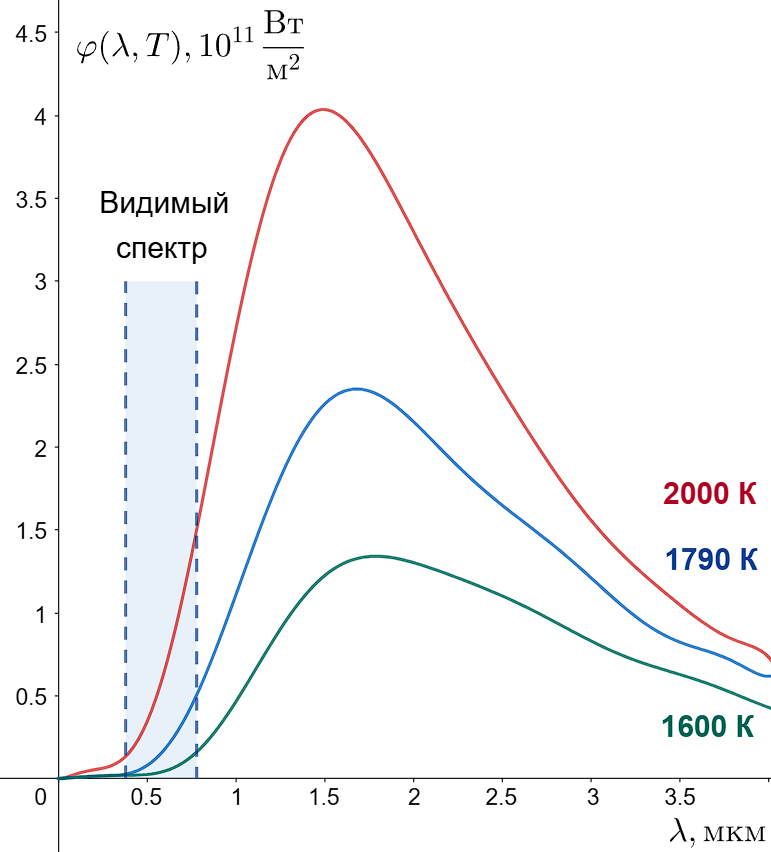
\includegraphics[width=7cm]{physics3/images/physics3_kirchhoff_law_functions}
\end{wrapfigure}

Физик Густав Кирхгофа на основе наблюдений выразил закон Кирхгофа: отношение испускательной и поглощательной способности не зависит от природы тела, оно является для всех тел одной и той же функцией частоты и температуры

\[\left(\frac{r_{\omega T}}{\alpha_{\omega T}}\right)_1 = \left(\frac{r_{\omega T}}{\alpha_{\omega T}}\right)_2 = \dots = \left(\frac{r_{\omega T}}{\alpha_{\omega T}}\right)_n = f(\omega, T)\]

Для абсолютно черного тела $f(\omega, T) = r_{\omega T}$

Далее экспериментально были получены кривые функций $\varphi(\lambda, T) = f\left(2\pi \frac{c}{\lambda}, T\right)$ для разных температур для абсолютно черного тела

На ней можно заметить, что при высоких температурах (2300 - 3100 К) лишь малая часть теплового излучения лежит в видимом для человека спектре, что объясняет малый КПД лампы накаливания


Позже был сформулирован закон Стефана-Больцмана: $R_T = \int_0^\infty r_{\omega T} d\omega = \int_0^\infty f(\omega, T) d\omega = \sigma T^4$, где $\sigma = 5.67 \cdot 10^{-8} \frac{\text{Вт}}{\text{м}^2 \cdot \text{К}^4}$ -- постоянная Стефана-Больцмана

Таким образом, можно вычислить мощность света от Солнца, попадающего на квадратный метр площадки на Земле и получить примерно $130 \frac{\text{Вт}}{\text{м}^2}$

Из этого появился закон Вина, который гласит, что максимум спектральной плотности энергетической светимости обратно пропорционален абсолютной температуре $\lambda_{\max} = \frac{b}{T}$, где $b = 2.9 \cdot 10^{-3} \text{м}\cdot\text{К}$ -- постоянная Вина

Функцию $f(\omega, T)$ пытались представить аналитически. Физики Рэлей и Джинс сформировали формулу Рэлея-Джинса: $f(\omega, T) = \frac{\omega^2}{4\pi^2 c^2} kT$. Эта формула хорошо сходится для больших длин волн, но плохо для маленьких в ультрафиолетовом спектре, так как $\int_0^\infty \frac{\omega^2}{4\pi^2 c^2} kT d\omega = \infty$ -- этот результат получил название ультрафиолетовой катастрофы

Позже Макс Планк высказал гипотезу Планка: электромагнитное излучение испускается телами не непрерывно, а в виде отдельных порций энергии (квантов), величина которых равна 

\[\varepsilon = h \nu = \frac{h c}{\lambda} = \hbar \omega,\]

где $h = 6.63 \cdot 10^{34} \text{Дж}\cdot\text{с}$ -- постоянная Планка, $\hbar = \frac{h}{2\pi} = 1.05 \cdot 10^{34} \text{Дж}\cdot\text{с}$ -- постоянная Планка с чертой

Энергия излучения получается, как сумма порций энергий $\varepsilon_n = n \hbar \omega$, где $n \in \Natural$

При $\frac{\hbar \omega}{kT} \gg 1$ (область высоких частот) получаем $f(\omega, T) = \frac{\omega^3}{4\pi^2 c^2} \frac{1}{1 + \frac{\hbar \omega}{kT} - 1} = \frac{\omega^3}{4\pi^2 c^2} kT$ -- формула Рэлея-Джинса

При $\frac{\hbar \omega}{kT} \ll 1$ (область низких частот) получаем $f(\omega, T) = \frac{\omega^3}{4\pi^2 c^2} e^{-\frac{\hbar \omega}{k T}} = \omega^2 \cdot F\left(\frac{\omega}{T}\right)$ -- формула Вина

Для абсолютно черного тела $R_T = \int_0^\infty \frac{\hbar}{4\pi^2 c^2} \frac{\omega^3 d\omega}{e^{-\frac{\hbar \omega}{k T}} - 1} = \frac{\pi^2 k^4}{60 c^2 \hbar^3} T^4 = \sigma T^4$ -- закон Стефана-Больцмана

\smallvspace 

Исследуем формулу Планка на экстремум, возьмем $\frac{d \varphi(\lambda, T)}{d\lambda} = 0$, получим трансцендентное уравнение $x e^x - 5(e^x - 1) = 0$, решением которого является $\frac{2\pi \hbar c}{k T \lambda_{\max}} = 4.965$, отсюда получаем закон смещения Вина: $T \lambda_m = \frac{2\pi \hbar c}{4.965 k} = b$

\bigvspace

Фотоэффект -- эффект, при котором электроны двигаются в веществе под действием светового излучения

Различают 3 типа фотоэффекта:

\begin{itemize}
    \item Внешний -- электрон покидает вещество. На основе внешнего фотоэффекта работают фотоэлементы
    
    Внешний фотоэффект создается так: помещаются фотокатод и анод в прозрачную колбу и откачивают воздух. При попадании света на фотокатод электроны переносятся с него на анод, создавая ток 

    \item Внутренний -- перераспределение электронов внутри чистого полупроводника под действием света. На внутреннем фотоэффекте основаны фоторезисторы

    \item Вентильный -- пропускание электроном через p-n переход при его обратном включении под действием света. На основе этого фотоэффекта работают фотодиоды
\end{itemize}


Наблюдения помогли понять, что при определенной длины волны фотоэффект резко прекращается. Чтобы выбить электрон из кристаллической решетки наружу, нужно сообщить ему энергию

Основные закономерности внешнего фотоэффекта отражены зависимостью величины фототока от напряжения между анодом и катодом. Такая зависимость называется вольт-амперной характеристикой: $I = I(U)$

% TODO картинка ВАХ

На вольт-амперной характеристике можно заметить две точки:

\begin{itemize}
    \item Напряжение, при котором тока нет. Его называют задерживающим (или запирающим) и оно обратного направления
    \item Ток насыщения, при котором выбивается максимально возможное число электронов из пластинки
\end{itemize}

\mediumvspace

Далее явление фотоэффекта изучал Столетов, который сформулировал первый закон фотоэффекта: сила фототока насыщения пропорциональная падающему световому потоку, то есть $I = \Phi$

Величина задерживающего напряжения позволяет определить максимальную скорость электронов

Второй закон фотоэффекта гласит, что задерживающее напряжение прямо пропорционально зависит от частоты: $U_\text{зап} = a\nu + b$, то есть $\tg \alpha = a = \const$

Третий закон фотоэффекта утверждает, что для каждого металла существует минимальная частота $\nu_{\text{кр}}$, при которой начинается фотоэффект

Часто длина волны такой частоты является красной, поэтому ее называют красной границей фотоэффекта

Разные металлы имеют различную частоту красной границы и одинаковую зависимость задерживающего напряжения от частоты

\mediumvspace

В 1905 году Альберт Эйнштейн объяснил второй закон тем, что металл поглощает свет порциями, то есть квантами. Тогда по формуле Планка $\varepsilon_{\text{фотона}} = h \nu$ получаем:

\fbox{$h \nu = A_{\text{выхода}} + E_{\text{кин. элект.}} = A_{\text{выхода}} + \frac{m v^2_{\max}}{2}$} -- уравнение Эйнштейна для фотоэффекта

\smallvspace

Здесь $A_{\text{выхода}}$ -- работа выхода, необходимая энергия для вытеснения электрона из вещества при температуре абсолютного нуля. Работа выхода для многих металлов находится в интервале от 1 до 10 эВ

При $v_{\max}$ получаем $\nu_\text{кр} = \frac{A_\text{вых}}{h}$

Также можем представить второй закон фотоэффекта так: $U_\text{зап} = \frac{h}{e} \nu - \frac{A_\text{вых}}{e}$

% end physics3_2025_09_15.tex

% begin physics3_2025_09_22.tex





% Увидеть результат фотоэффекта, то есть выбивание электрон, невооруженным глазом сложно. Однако можно соединить пластинки к источнику напряжения и увидеть силу тока чуть-чуть выше из-за фотоэффекта

\section{Давление света}

Фотоны, частицы света, имеют массу покоя равную нулю, движутся в вакууме со скоростью $c = 3 \cdot 10^8$, имеют энергию и импульс

Энергия фотона зависит от частоты света: $\varepsilon = h \nu = \hbar \omega = \frac{h c}{\lambda}$

Из специальной теории относительности нам известна формула связи энергии с массой и скоростью: $E^2 = m^2 c^4 + p^2 c^2$. Если тело покоится, то его энергия равна $E^2 = p^2 c^2$. Если масса равна нуля $E^2 = p^2 c^2$ или $E = p c$

Тогда импульс (то есть мера количества движения) фотона равен $p = \frac{\varepsilon}{c} = \frac{h \nu}{c} = \frac{h}{\lambda}$

Рассмотрим такую модель: электромагнитная волна падает на металлическую пластину. Пластина содержит свободные электроны, которые двигаются циклично из-за электрического поля в волне, а магнитное поле создает 

Свет, падая на поверхность, создает давление. В общем случае, часть фотонов отражается от поверхности, а часть поглощается

Давление света определяется импульсом, который передается поверхности фотонами, падающими на поверхность за время наблюдения

\[P = \frac{F}{S} = \frac{\Delta p}{S \Delta t}\]

При отражении импульс фотона меняется на $2 \frac{h}{\lambda}$ (так как направление становится противоположным), а при поглощении -- на $\frac{h}{\lambda}$

Пусть $\alpha$ -- коэффициент отражения, тогда $\alpha N$ фотонов отразится, а $(1 - \alpha) N$ -- поглотится

Полное изменение импульса равно $\Delta p = \alpha 2\frac{h}{\lambda} N + (1 - \alpha) \frac{h}{\lambda} N$ или $\Delta p = (1 + \alpha) \frac{h}{\lambda} N$

Количество фотонов, падающих на поверхность, можно выразить так: $N = n S c \Delta t$

Тогда давление $P = (1 + \alpha) n \frac{h c}{\lambda} = (1 + \alpha) n h v$

Введем другую переменную $w = n h \nu$ -- объемная плотность световой энергии, тогда $P = (1 + \alpha) w$

Так как $w = \frac{I}{c}$, $P = (1 + \alpha) \frac{I}{c}$, то есть световое давление определяется энергией (интенсивностью света)

Общее давление солнечных лучей на Землю равно $4.3$ мкПа, поэтому в земных условиях заметить величину светового давления тяжело. Впервые давление света измерил физик Лебедев в 1899 году

\mediumvspace

В 1922 году физик Комптон изучал взаимодействие рентгеновского излучения с парафином и графита и наблюдал дифракционные картины рассеянного излучения

Предполагалось, согласно классической волновой теории рассеяния ЭМИ, что длина волны волны не должна изменяться

Под действием периодического электрического поля электромагнитной волны электрон вещества должен колебаться с частотой поля. Поэтому рассеянные веществом вторичные волны должны иметь ту же частоту, что и первичное излучение

% TODO картинка

Рассеянное рентгеновское излучение состояло не только из компонент с исходной длины волны $\lambda$, но и из компоненты с другой длиной волны $\lambda^\prime$, которые рассеивались под другим углом

Подобное явление получило название эффекта Комптона -- явление упругого рассеяния электромагнитного излучения на свободных электронах вещества, сопровождающееся увеличением длины волны. Дело в том, что при столкновении фотона с электроном фотон теряет часть импульса, которая передается электрону, таким образом, фотон меняет длину волны

Сдвиг волны составляет $\Delta \lambda = \lambda_K (1 - \cos\varphi)$, где $\varphi$ -- угол отклонения вторичной волны, а $\lambda_K = \frac{h}{m_{\text{пок}} c} = 2.426$ пм -- Комптоновская длина волны

\mediumvspace

Таким образом, в разных опытах свет ведет себя по-разному. Явления интерференции, дифракции, поляризации, дисперсии объясняются электромагнитной волновой природой света. В тепловом излучении, фотоэффекте, эффекте Комптона, давления света свет представляется как поток частиц

Поэтому свет обладает двойственностью: он является и частицей и волной. Тогда Луи де Бройль в 1924 году выдвинул гипотезу, что частицы вещества наряду с корпускулярными свойствами обладают свойствами волны

Тогда $\lambda = \frac{h}{p} = \frac{h}{mv}$ (а в релятивистском случае $p = \frac{mv}{\sqrt{1 - \frac{v^2}{c^2}}}$)

А это значит, что маленькие частицы, такие как электроны, протоны, нейтроны, могут обладать длиной волны

С помощью этого можно измерить период решетки: направляя пучок электронов с известной скоростью (а значит известной длиной волны де Бройля) на монокристалл, измерив углы дифракции, можем получить период по формуле $d \sin \varphi = k \lambda$


% end physics3_2025_09_22.tex



\end{document}

